%! Author = jimmyt
%! Date = 1/15/23

% Preamble
\documentclass[11pt]{article}

% Packages
\usepackage{amsmath}
\usepackage[margin=1in]{geometry}
\usepackage{longtable}
\usepackage{multirow}
\usepackage{tikz}

%\usepackage{showframe}

\usetikzlibrary{positioning}

\author{jimmyt}

% Document
\begin{document}

    \title{Commuto}
    \maketitle

    \begin{abstract}
    Commuto is a collection of software allowing private, noncustodial, censorship resistant
    exchange of national currencies and tokens adopting the ERC20\cite{ERC20} standard on
    Ethereum Virtual Machine\cite{Ethereum} compatible blockchains.
    The Commuto Protocol's name comes from the Latin word ``commuto'', meaning ``I exchange'' or ``I
    barter.''
    \end{abstract}

    \section*{Introduction}

    Commuto is primarily composed of two software components: a set of smart contracts deployed on
    an EVM-compatible blockchain, and a set of applications that can interact both with said
    on-chain contracts as well as other Commuto users.
    The smart contracts will be referred to henceforth as ``Commuto Core'' and said applications
    will be referred to as ``Commuto Interfaces''.
    An intention expressed by a Commuto user to buy or sell a particular ERC20 token in exchange for
    one or more particular national currency is known as an ``offer''.
    An exchange of national currency and ERC20 tokens between two users is known as a ``swap''.

    Because Commuto allows users to exchange national currency, certain pieces of private
    information (such as bank account details and addresses) must be exchanged between users.
    Additionally, users should be able to communicate with each other in a convenient manner, in
    order to resolve any problems that may arise during the swap process.
    While an EVM blockchain (on which Commuto Core contracts are deployed could) theoretically
    be used to exchange such information by storing it (even if only temporarily) on-chain, the
    relatively high cost of storage on such blockchains makes this approach unfeasible.
    Additionally, many users are likely accustomed to instant messaging applications that
    deliver messages in less than a second.
    The relatively longer time required to incorporate a new transaction into a such blockchain is
    yet another reason why an EVM-blockchain-based communication system between users is not
    practical.
    Therefore, Commuto Interfaces use Matrix\cite{Matrix} to reliably exchange information in a
    decentralized, censorship-resistant manner.
    Matrix is a network of nodes running software conforming to the Matrix
    Specification\cite{MatrixSpec}, which defines a set of open APIs for decentralised
    communication, suitable for securely publishing, persisting and subscribing to data over a
    global open federation of servers with no single point of control.
    A Matrix Room is a directed acyclic graph of Events, the ordering of which is the chronological
    ordering of Events in the room.
    Any node may maintain a copy of any such Room, and nods may add new elements to Rooms.
    Events are simply JSON objects with zero or more ``parent'' events, which are chronological
    predecessors in the event graph.
    Nodes use state resolution algorithms and communicate with one another using federation
    algorithms (as defined in the specification) in order to maintain persistent,
    eventually-consistent synchronization of Room state across all nodes in the network.
    Therefore, no single node (referred to in the Matrix Specification and henceforth in this paper
    as a ``homeserver'') has control over any given Room.
    Thus, due to its open, flexible, decentralized, censorship-resistant nature, Commuto uses Matrix
    to exchange data between Commuto Interfaces.

    \section*{Commuto Core}

    Commuto Core is composed of smart contracts that enable swaps between offer makers and offer
    takers, and also allow the resolution of disputes between makers and takers.
    (For example a dispute may arise when a token buyer claims to have sent payment to the seller,
    but the seller claims that they have not received this payment.)
    We begin by considering the operations of the CommutoSwap smart contract, which enables the
    swapping process.
    Subsequently, we explain the functionality of the contracts allowing dispute resolution,
    governance, and the distribution of service fees collected by CommutoSwap.
    Smart contract code snippets are written in Solidity\cite{Solidity}.
    For readability, we include parameter names in function signatures, even though actual EVM smart
    contract function signatures do not include parameter names.

    \subsection*{CommutoSwap}

    The CommutoSwap smart contract can be best understood by considering the steps of the swap
    process, so we describe it in this context.
    Note that, as described in the introduction, the swap process includes the exchange of
    information via Matrix.
    However, because this section focuses on the operations of CommutoSwap, we temporarily omit the
    details of off-blockchain communication, and instead describe them in a later section.
    Throughout this document, we use the symbol ERC to refer to any ERC20 token, and a the symbol
    CUR to refer to any national currency.
    Sellers have ERC and want CUR, and buyers have CUR and want ERC.

    \subsubsection*{Opening an Offer}

    An offer maker opens an offer by calling the \verb|openOffer| function.
    This function has the following signature:
    \begin{verbatim}
    openOffer(bytes16 offerID, Offer newOffer)
    \end{verbatim}
    where \verb|offerID| is a Version-4 UUID\cite{UUID}, and \verb|newOffer| is an \verb|Offer|
    struct that is defined as follows:
    \begin{verbatim}
    struct Offer {
        bool isCreated
        bool isTaken
        address maker
        bytes interfaceId
        address stablecoin
        uint256 amountLowerBound
        uint256 amountUpperBound
        uint256 securityDepositAmount
        uint256 serviceFeeRate
        SwapDirection direction
        bytes[] settlementMethods
        uint256 protocolVersion }
    \end{verbatim}
    and \verb|SwapDirection| is an \verb|enum| that is defined as follows:
    \begin{verbatim}
    enum SwapDirection {
        BUY
        SELL
    }
    \end{verbatim}
    A \verb|SwapDirection.BUY| value indicates that the maker of the Offer is a buyer, as previously
    defined, and \verb|SwapDirection.SELL| is similar.
    The properties of the \verb|Offer| struct are as follows: \\

    \begin{longtable}[p]{ |p{2.5cm}|p{4cm}|p{7cm}| }
    \hline
    \multicolumn{3}{|c|}{Offer} \\
    \hline
    Property Type & Property Name & Description \\
    \hline
    bool & isCreated & Used by contract code to check for offer existence, will be set to true
    by \verb|openOffer|. \\
    bool & isTaken & Used by contract code to check whether an offer is taken, will be set to
    false by \verb|openOffer|. \\
    address & maker & The maker's address, will be sent to \verb|msg.sender| by \verb|openOffer|. \\
    bytes & interfaceId & An array of bytes that should be placed in the ``recipient'' field of any
    message sent to the maker of this offer via Matrix. \\
    address & stablecoin & The contract address of the token that the offer maker is offering to
    swap. \\
    uint256 & amountLowerBound & The lower bound on the range of token amounts that the maker is
    willing to swap. \\
    uint256 & amountUpperBound & The upper bound on the range of token amounts that the maker is
    willing to swap. \\
    uint256 & securityDepositAmount & The token amount to be used as a security deposit, which must
    not be less than ten percent of amountUpperBound. \\
    uint256 & serviceFeeRate & The percentage times 100 of the amount of swapped tokens that the
    maker and taker must pay as a service fee. \\
    SwapDirection & direction & Indicates whether the maker is offering to buy tokens or sell
    tokens. \\
    bytes[] & settlementMethods & An array of \verb|bytes|, each one representing a method by which
    the maker is willing to send/receive payment for tokens. \\
    uint256 & protocolVersion & A number optionally describing which version of the Commuto
    Interface software was used to open this offer. \\
        \hline
    \end{longtable}

    \pagebreak
    When called, \verb|openOffer| does the following: \\

    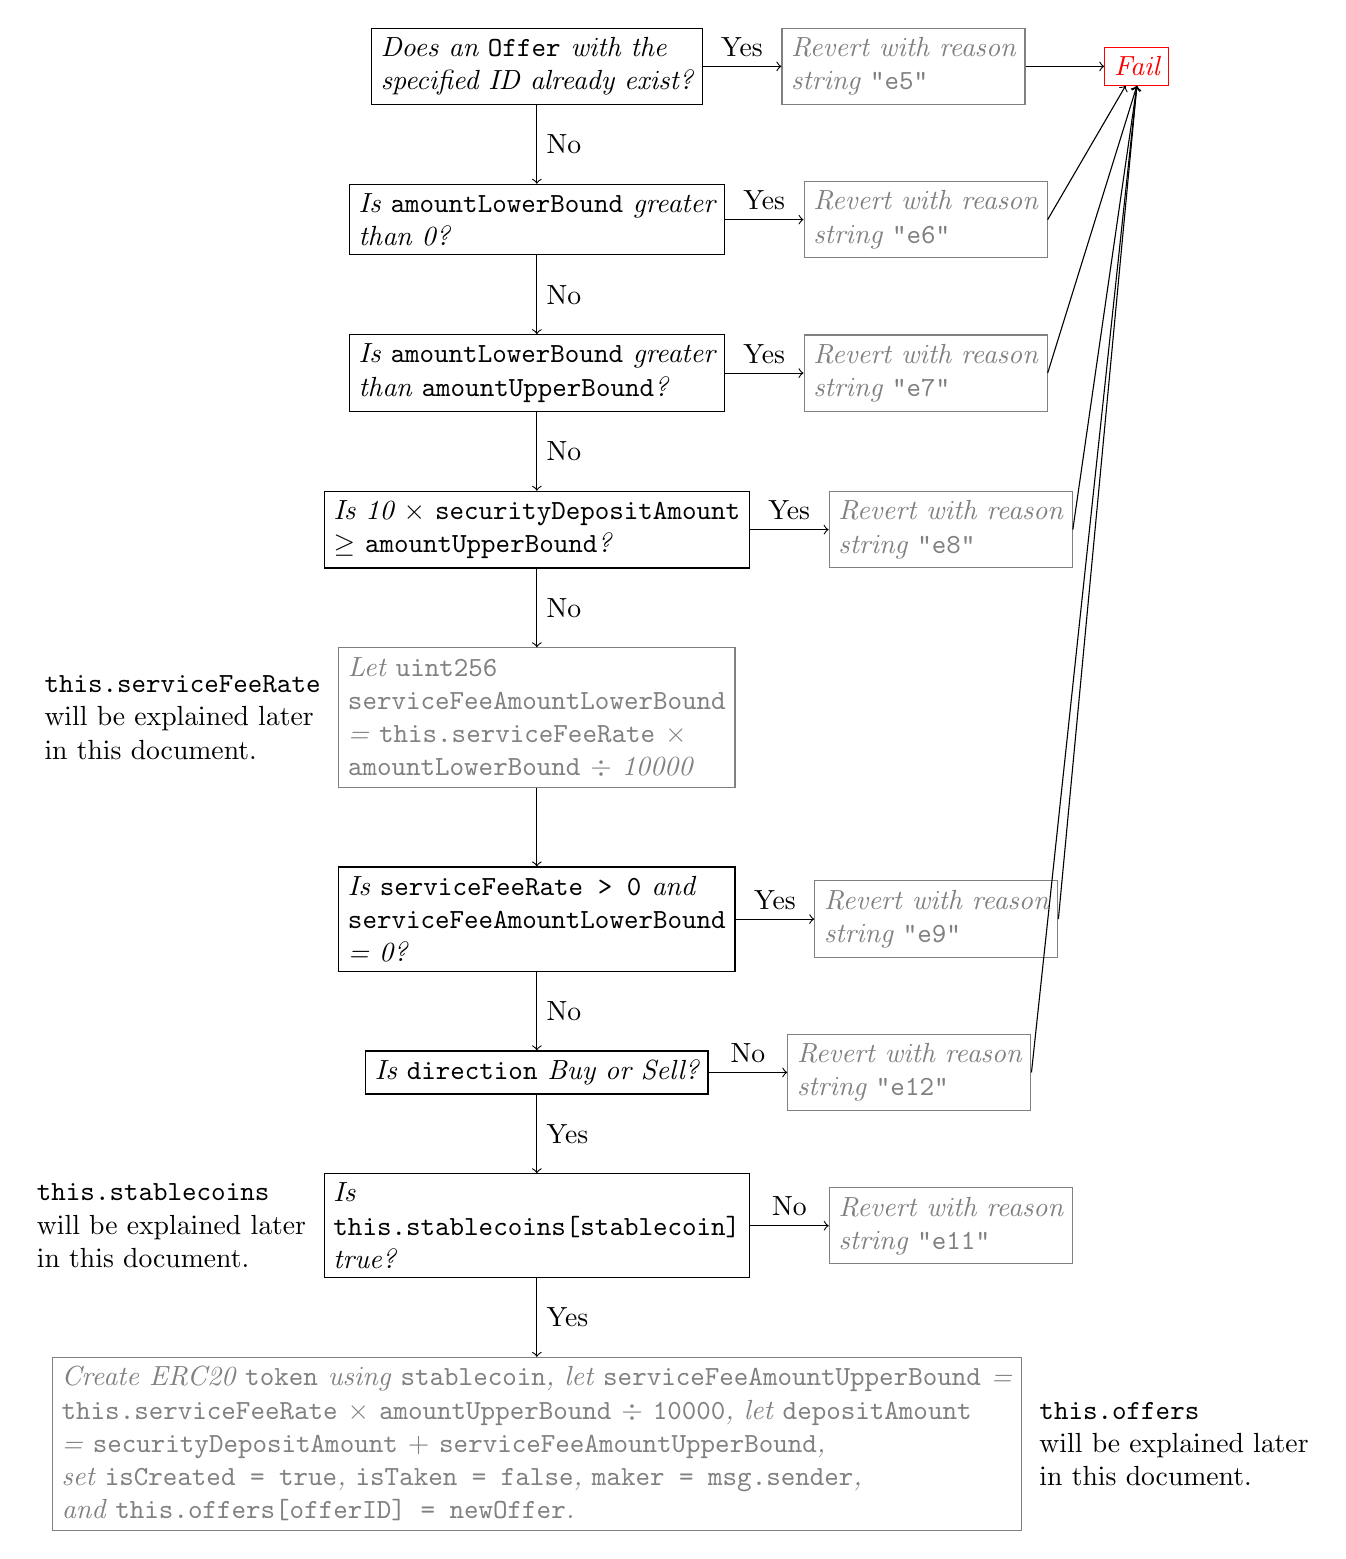
\begin{tikzpicture}[
        question/.style={
            % The shape
            rectangle,
            % The border
            thin,
            draw = black!100,
            % The color
            color = black,
            % Font
            font = \itshape
        },
        action/.style={
            % The shape
            rectangle,
            % The border
            thin,
            draw = gray!100,
            % The color
            color = gray,
            % Font
            font = \itshape
        },
        fail/.style={
            % The shape
            rectangle,
            % The border
            thin,
            draw = red!100,
            % The color
            color = red,
            % Font
            font = \itshape
        },
    ]
        \node (isCreated) [question,align=left] {Does an \verb|Offer| with the \\ specified ID
        already exist?};
        \node (revert_e5) [action,align=left,right=of isCreated] {Revert with reason \\ string
        \verb|"e5"|};
        \path (isCreated) edge[->] node[pos=0.5,above] {Yes} (revert_e5);
        \node (fail) [fail,right=of revert_e5] {Fail};
        \path (revert_e5) edge[->] (fail);

        \node (sufficientAmount) [question,align=left,below=of isCreated] {Is
        \verb|amountLowerBound| greater \\ than 0?};
        \path (isCreated) edge[->] node[pos=0.5,right] {No} (sufficientAmount);
        \node (revert_e6) [action,align=left,right=of sufficientAmount] {Revert with reason \\
        string \verb|"e6"|};
        \path (sufficientAmount) edge[->] node[pos=0.5,above] {Yes} (revert_e6);
        \path (revert_e6.east) edge[->] (fail);

        \node (properRange) [question,align=left,below=of sufficientAmount ] {Is
        \verb|amountLowerBound| greater \\ than \verb|amountUpperBound|?};
        \path (sufficientAmount) edge[->] node[pos=0.5,right] {No} (properRange);
        \node (revert_e7) [action,align=left,right=of properRange] {Revert with reason \\ string
        \verb|"e7"|};
        \path (properRange) edge[->] node[pos=0.5,above] {Yes} (revert_e7);
        \path (revert_e7.east) edge[->] (fail.south);

        \node (sufficientSecurityDeposit) [question,align=left,below=of properRange] {Is 10 $\times$ \verb|securityDepositAmount| \\ $\geq$ \verb|amountUpperBound|?};
        \path (properRange) edge[->] node[pos=0.5,right] {No} (sufficientSecurityDeposit);
        \node (revert_e8) [action,align=left,right=of sufficientSecurityDeposit] {Revert with reason \\ string \verb|"e8"|};
        \path (sufficientSecurityDeposit) edge[->] node[pos=0.5,above] {Yes} (revert_e8);
        \path (revert_e8.east) edge[->] (fail.south);

        \node (calculateServiceFeeAmntLow) [action,align=left,below=of sufficientSecurityDeposit] {Let \verb|uint256| \\ \verb|serviceFeeAmountLowerBound| \\ = \verb|this.serviceFeeRate| $\times$ \\ \verb|amountLowerBound| $\div$ 10000};
        \path (sufficientSecurityDeposit) edge[->] node[pos=0.5,right] {No} (calculateServiceFeeAmntLow);
        \node (serviceFeeRateDisclaimer) [align=left,left=1mm of calculateServiceFeeAmntLow] {\verb|this.serviceFeeRate| \\ will be explained later \\ in this document.};

        \node (sufficientServiceFee) [question,align=left,below=of calculateServiceFeeAmntLow] {Is \verb|serviceFeeRate > 0| and \\ \verb|serviceFeeAmountLowerBound| \\ = 0?};
        \path (calculateServiceFeeAmntLow) edge[->] (sufficientServiceFee);
        \node (revert_e9) [action,align=left,right=of sufficientServiceFee] {Revert with reason \\ string \verb|"e9"|};
        \path (sufficientServiceFee) edge[->] node[pos=0.5,above] {Yes} (revert_e9);
        \path (revert_e9.east) edge[->] (fail.south);

        \node (validDirection) [question,align=left,below=of sufficientServiceFee] {Is \verb|direction| Buy or Sell?};
        \path (sufficientServiceFee) edge[->] node[pos=0.5,right] {No} (validDirection);
        \node (revert_e12) [action,align=left,right=of validDirection] {Revert with reason \\ string \verb|"e12"|};
        \path (validDirection) edge[->] node[pos=0.5,above] {No} (revert_e12);
        \path (revert_e12.east) edge[->] (fail.south);

        \node (validToken) [question,align=left,below=of validDirection] {Is \\ \verb|this.stablecoins[stablecoin]| \\ true?};
        \path (validDirection) edge[->] node[pos=0.5,right] {Yes} (validToken);
        \node (stablecoinsNote) [align=left,left=1mm of validToken] {\verb|this.stablecoins| \\ will be explained later \\ in this document.};
        \node (revert_e11) [action,align=left,right=of validToken] {Revert with reason \\ string \verb|"e11"|};
        \path (validToken) edge[->] node[pos=0.5,above] {No} (revert_e11);

        \node (openOffer) [action,align=left,below=of validToken] {
            Create ERC20 \verb|token| using \verb|stablecoin|, let \verb|serviceFeeAmountUpperBound|
            = \\ \verb|this.serviceFeeRate| $\times$ \verb|amountUpperBound| $\div$ \verb|10000|,
            let \verb|depositAmount| \\ = \verb|securityDepositAmount| $+$
            \verb|serviceFeeAmountUpperBound|, \\ set \verb|isCreated = true|,
            \verb|isTaken = false|, \verb|maker = msg.sender|,\\ and
            \verb|this.offers[offerID] = newOffer|.

        };
        \node (offersNote) [align=left,right=1mm of openOffer] {\verb|this.offers| \\ will be explained later \\ in this document.};
        \path (validToken) edge[->] node[pos=0.5,right] {Yes} (openOffer);

    \end{tikzpicture}

    Continued on next page.

    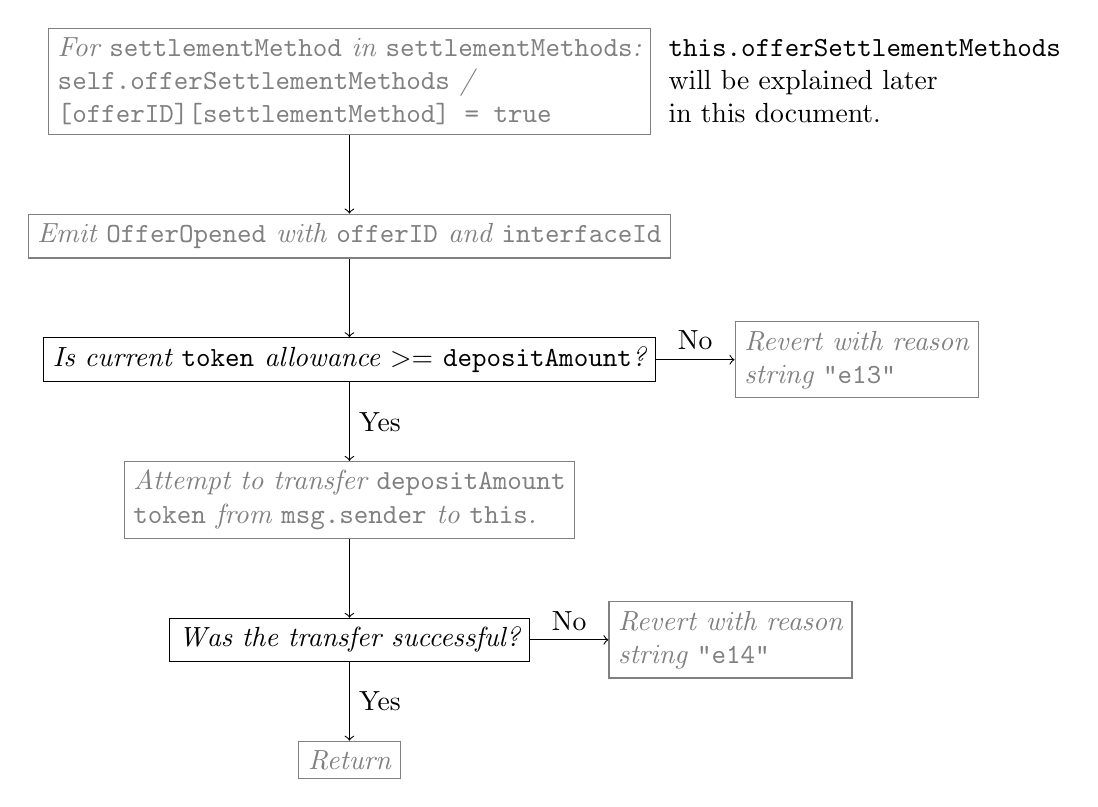
\begin{tikzpicture}[
        question/.style={
            rectangle, thin, draw = black!100, color = black, font = \itshape
        },
        action/.style={
            rectangle, thin, draw = gray!100, color = gray, font = \itshape
        },
    ]
    \node (addSettlementMethods) [action,align=left] {
        For \verb|settlementMethod| in \verb|settlementMethods|: \\
        \verb|self.offerSettlementMethods| / \\
        \verb|[offerID][settlementMethod] = true|
    };
    \node (addSettlementMethodsNote) [align=left,right=1mm of addSettlementMethods] {\verb|this.offerSettlementMethods| \\ will be explained later \\ in this document.};

    \node (emitEvent) [action, below=of addSettlementMethods] { Emit \verb|OfferOpened| with \verb|offerID| and \verb|interfaceId| };
    \path (addSettlementMethods) edge[->] (emitEvent);

    \node (verifyAllowance) [question, below=of emitEvent] { Is current \verb|token| allowance $>=$ \verb|depositAmount|? };
    \path (emitEvent) edge[->] (verifyAllowance);
    \node (revert_e13) [action,align=left,right=of verifyAllowance] {Revert with reason \\ string \verb|"e13"|};
    \path (verifyAllowance) edge[->] node[pos=0.5,above] {No} (revert_e13);

    \node (attemptTransfer) [action,align=left,below=of verifyAllowance] { Attempt to transfer \verb|depositAmount| \\ \verb|token| from \verb|msg.sender| to \verb|this|. };
    \path (verifyAllowance) edge[->] node[pos=0.5,right] {Yes} (attemptTransfer);

    \node (verifyTransfer) [question,below=of attemptTransfer] {Was the transfer successful?};
    \path (attemptTransfer) edge[->] (verifyTransfer);
    \node (revert_e14) [action,align=left,right=of verifyTransfer] {Revert with reason \\ string \verb|"e14"|};
    \path (verifyTransfer) edge[->] node[pos=0.5,above] {No} (revert_e14);
    \node (return) [action,below=of verifyTransfer] {Return};
    \path (verifyTransfer) edge[->] node[pos=0.5,right] {Yes} (return);

    \end{tikzpicture}

    \verb|this.serviceFeeRate| is a property of the CommutoSwap contract of type \verb|uint256|,
    expressed as a percentage times one hundred, of the amount of tokens exchanged between a buyer
    and seller, that both the buyer and seller must pay as a service fee.

    \verb|this.serviceFeeRate| is a property of the CommutoSwap contract, and is a mapping from
    \verb|address|es to \verb|bool| values.
    Offers to exchange a token can be created if and only if \verb|this.serviceFeeRate| maps the
    address of the token to \verb|true|.

    \verb|this.offers| is a property of the CommutoSwap contract, and is a mapping from
    \verb|bytes16| values to \verb|Offer|s.

    \verb|this.offerSettlementMethods| is a nested mapping.
    The outer mapping maps \verb|bytes16| to inner mappings, and an inner mapping maps \verb|bytes|
    to \verb|bool| values.

    \verb|OfferOpened| is an Event with the following signature:
    \begin{verbatim}
    OfferOpened(bytes16 offerID, bytes interfaceId)
    \end{verbatim}

    \subsubsection*{Taking an Offer}

    An offer taker takes an existing offer by calling the \verb|takeOffer| function.
    This function has the following signature:
    \begin{verbatim}
    takeOffer(bytes16 offerID, Swap newSwap)
    \end{verbatim}
    where \verb|offerID| is a Version-4 UUID and newSwap is a \verb|Swap| struct that is defined as
    follows:
    \begin{verbatim}
    struct Swap {
        bool isCreated;
        bool requiresFill;
        address maker;
        bytes makerInterfaceId;
        address taker;
        bytes takerInterfaceId;
        address stablecoin;
        uint256 amountLowerBound;
        uint256 amountUpperBound;
        uint256 securityDepositAmount;
        uint256 takenSwapAmount;
        uint256 serviceFeeAmount;
        uint256 serviceFeeRate;
        SwapDirection direction;
        bytes settlementMethod;
        uint256 protocolVersion;
        bool isPaymentSent;
        bool isPaymentReceived;
        bool hasBuyerClosed;
        bool hasSellerClosed;
        DisputeRaiser disputeRaiser;
    }
    \end{verbatim}
    and \verb|DisputeRaiser| is an \verb|enum| that is defined as follows:
    \begin{verbatim}
    enum DisputeRaiser  {
        NONE,
        MAKER,
        TAKER
    }
    \end{verbatim}
    The meaning of these values and the use of the \verb|Swap.disputeRaiser| property will be
    described later in this paper.
    The properties of the \verb|Swap| struct are as follows:
    \begin{longtable}[p]{ |p{2.5cm}|p{4cm}|p{7cm}| }
        \hline
        \multicolumn{3}{|c|}{Swap} \\
        \hline
        Property Type & Property Name & Description \\
        \hline
        bool & isCreated & Used by contract code to check for swap existence, will be set to true by \verb|takeOffer|. \\
        bool & requiresFill & If the maker of this swap is the token seller, this indicates whether the seller has transferred to CommutoSwap the amount of tokens that they are selling.
            If the maker of this swap is not the token seller, this is not used. \\
        address & maker & Identical to \verb|Offer.maker| of the offer being taken. \\
        bytes & makerInterfaceId & Identical to \verb|Offer.interfaceId| of the offer being taken. \\
        address & taker & The taker's address, will be sent to \verb|msg.sender| by \verb|takeOffer|. \\
        bytes & takerInterfaceId & An array of bytes that should be placed in the “recipient” field of
            any message sent to the taker of this offer via Matrix. \\
        address & stablecoin & Identical to \verb|Offer.stablecoin| of the offer being taken. \\
        uint256 & amountLowerBound & Identical to \verb|Offer.amountLowerBound| of the offer being taken. \\
        uint256 & amountUpperBound & Identical to \verb|Offer.amountUpperBound| of the offer being taken. \\
        uint256 & securityDepositAmount & Identical to \verb|Offer.securityDepositAmount| of the offer being taken. \\
        uint256 & takenSwapAmount & The exact amount of tokens that will be exchanged between the maker and the taker.
            Must be such that \verb|amountLowerBound| $\leq$ takenSwapAmount $\leq$ \verb|amountUpperBound|. \\
        uint256 & serviceFeeAmount & Used by contract code, will be set to \verb|Offer.serviceFeeRate| of the offer being taken $\times$ \verb|takenSwapAmount| $\div$ \verb|10000|.\\
        uint256 & serviceFeeRate & Identical to \verb|Offer.serviceFeeRate| of the offer being taken. \\
        SwapDirection & direction & Identical to \verb|Offer.direction| of the offer being taken. \\
        bytes & settlementMethod & A \verb|bytes| value representing the method by which the buyer will send payment for the exchanged tokens.
            Must be equal to one of the elements in the \verb|Offer.settlementMethods| array of the offer being taken. \\
        uint256 & protocolVersion & Identical to \verb|Offer.protocolVersion| of the offer being taken. \\
        bool & isPaymentSent & Indicates whether the buyer has sent payment for tokens purchased.
            Will be set to false by \verb|takeOffer|. \\
        bool & isPaymentReceived & Indicates whether the seller has received payment for tokens sold.
            Will be set to false by \verb|takeOffer|. \\
        bool & hasBuyerClosed & Indicates whether the buyer has closed the swap to reclaim their security deposit (and unused service fee amount, if they are the maker).
            Will be set to false by \verb|takeOffer|. \\
        bool & hasSellerClosed & Indicates whether the seller has closed the swap to reclaim their security deposit (and unused service fee amount, if they are the maker).
            Will be set to false by \verb|takeOffer|. \\
        DisputeRaiser & disputeRaiser & Indicates whether the buyer, seller, or neither has raised a dispute during the swap process.
            Will be set to \verb|NONE| by \verb|takeOffer|. \\
        \hline
    \end{longtable}

    When called, \verb|takeOffer| does the following:

    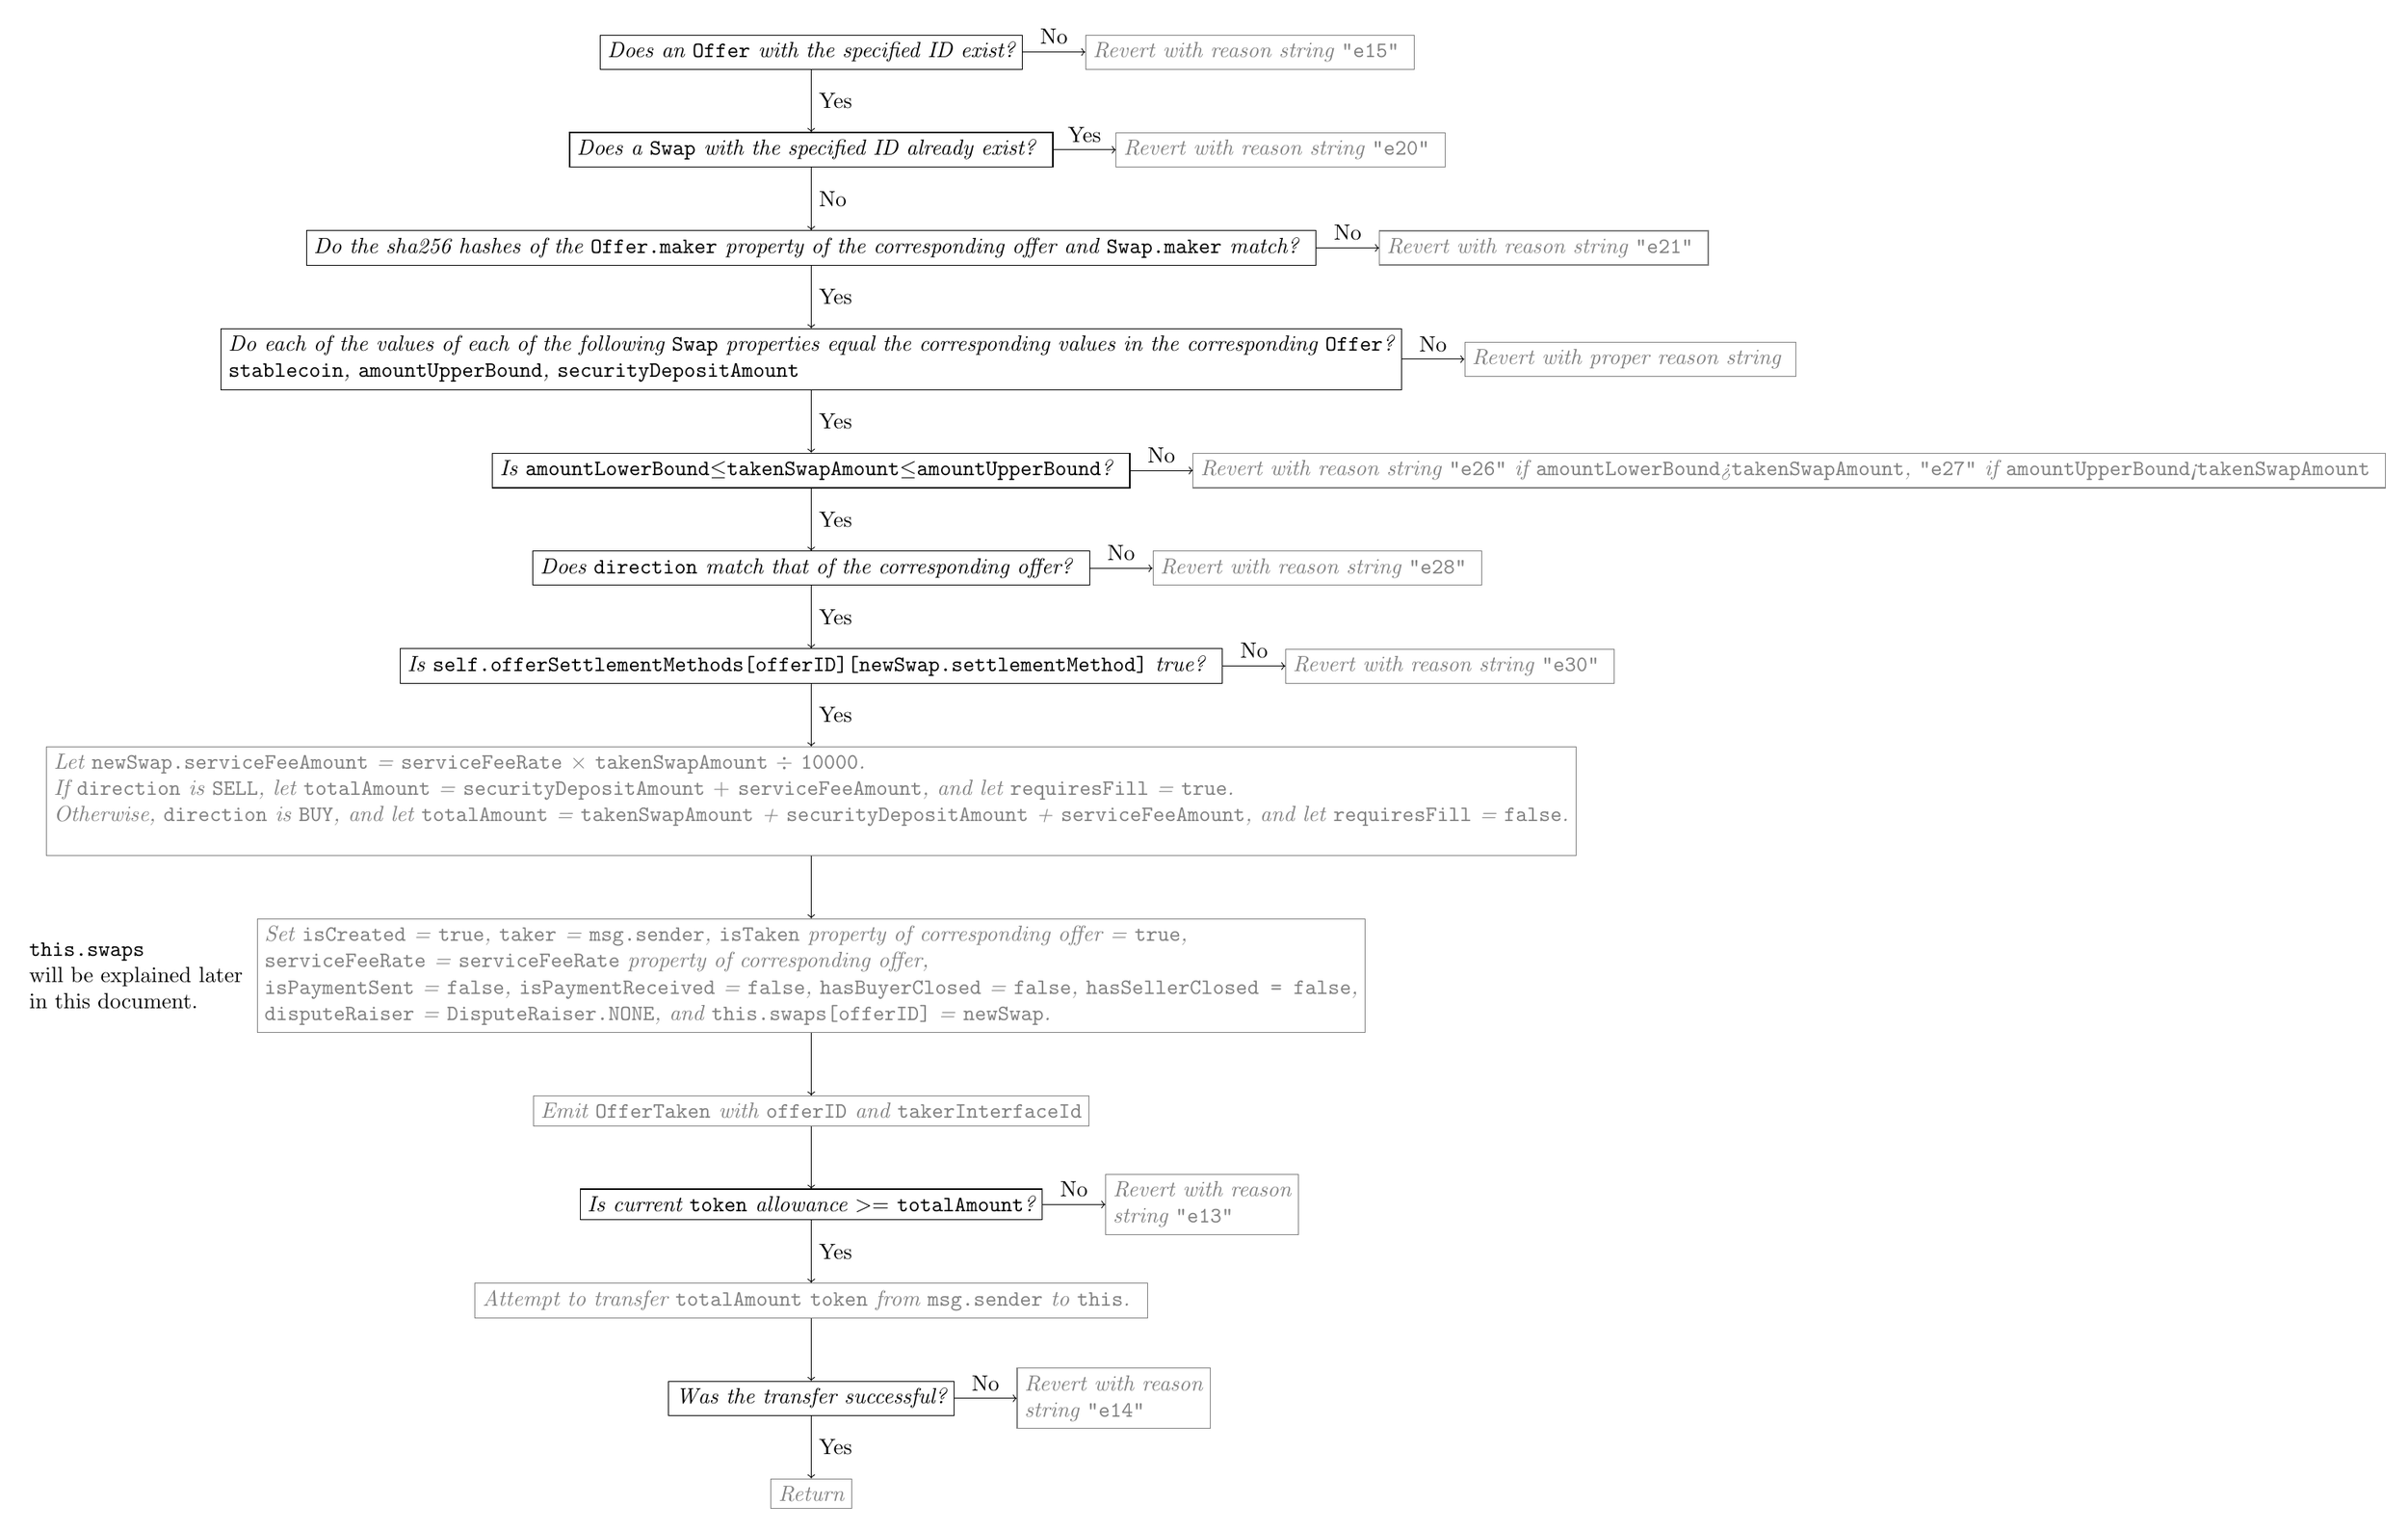
\begin{tikzpicture}[
        question/.style={
            rectangle, thin, draw = black!100, color = black, font = \itshape
        },
        action/.style={
            rectangle, thin, draw = gray!100, color = gray, font = \itshape
        },
    ]
        \node (isCreated) [question,align=left] { Does an \verb|Offer| with the specified ID exist?};
        \node (revert_e15) [action,align=left,right=of isCreated] { Revert with reason string \verb|"e15"| };
        \path (isCreated) edge[->] node[pos=0.5,above] {No} (revert_e15);

        \node (sufficientAmount) [question,align=left,below=of isCreated] { Does a \verb|Swap| with the specified ID already exist? };
        \path (isCreated) edge[->] node[pos=0.5,right] {Yes} (sufficientAmount);
        \node (revert_e20) [action,align=left,right=of sufficientAmount] { Revert with reason string \verb|"e20"| };
        \path (sufficientAmount) edge[->] node[pos=0.5,above] {Yes} (revert_e20);

        \node (matchingMakerID) [question,align=left,below=of sufficientAmount] { Do the sha256 hashes of the \verb|Offer.maker| property of the corresponding offer and \verb|Swap.maker| match? };
        \path (sufficientAmount) edge[->] node[pos=0.5,right] {No} (matchingMakerID);
        \node (revert_e21) [action,align=left,right=of matchingMakerID] { Revert with reason string \verb|"e21"| };
        \path (matchingMakerID) edge[->] node[pos=0.5,above] {No} (revert_e21);

        \node (matchingProperties1) [question,align=left,below=of matchingMakerID] {
            Do each of the values of each of the following \verb|Swap| properties equal the
            corresponding values in the corresponding \verb|Offer|? \\
            \verb|stablecoin|, \verb|amountUpperBound|, \verb|securityDepositAmount|
        };
        \path (matchingMakerID) edge[->] node[pos=0.5,right] {Yes} (matchingProperties1);
        \node (revert_proper1) [action,align=left,right=of matchingProperties1] { Revert with proper reason string };
        \path (matchingProperties1) edge[->] node[pos=0.5,above] {No} (revert_proper1);

        \node (amountInRange) [question,align=left,below=of matchingProperties1] { Is \verb|amountLowerBound|$\leq$\verb|takenSwapAmount|$\leq$\verb|amountUpperBound|? };
        \path (matchingProperties1) edge[->] node[pos=0.5,right] {Yes} (amountInRange);
        \node (revert_e26_e27) [action,align=left,right=of amountInRange] { Revert with reason string \verb|"e26"| if \verb|amountLowerBound|>\verb|takenSwapAmount|, \verb|"e27"| if \verb|amountUpperBound|<\verb|takenSwapAmount| };
        \path (amountInRange) edge[->] node[pos=0.5,above] {No} (revert_e26_e27);

        \node (matchingDirection) [question,align=left,below=of amountInRange] { Does \verb|direction| match that of the corresponding offer? };
        \path (amountInRange) edge[->] node[pos=0.5,right] {Yes} (matchingDirection);
        \node (revert_e28) [action,align=left,right=of matchingDirection] { Revert with reason string \verb|"e28"| };
        \path (matchingDirection) edge[->] node[pos=0.5,above] {No} (revert_e28);

        \node (settlementMethodSupported) [question,align=left,below=of matchingDirection] { Is \verb|self.offerSettlementMethods[offerID][newSwap.settlementMethod]| true? };
        \path (matchingDirection) edge[->] node[pos=0.5,right] {Yes} (settlementMethodSupported);
        \node (revert_e30) [action,align=left,right=of settlementMethodSupported] { Revert with reason string \verb|"e30"| };
        \path (settlementMethodSupported) edge[->] node[pos=0.5,above] {No} (revert_e30);

        \node (calculateAmounts) [action,align=left,below=of settlementMethodSupported] {
            Let \verb|newSwap.serviceFeeAmount| = \verb|serviceFeeRate| $\times$ \verb|takenSwapAmount| $\div$ \verb|10000|. \\
            If \verb|direction| is \verb|SELL|, let \verb|totalAmount| = \verb|securityDepositAmount| $+$ \verb|serviceFeeAmount|, and let \verb|requiresFill| = \verb|true|. \\
            Otherwise, \verb|direction| is \verb|BUY|, and let \verb|totalAmount| = \verb|takenSwapAmount| + \verb|securityDepositAmount| + \verb|serviceFeeAmount|, and let \verb|requiresFill| = \verb|false|. \\
        };
        \path (settlementMethodSupported) edge[->] node[pos=0.5,right] {Yes} (calculateAmounts);

        \node (setValues) [action,align=left,below=of calculateAmounts] {
            Set \verb|isCreated| = \verb|true|, \verb|taker| = \verb|msg.sender|,
            \verb|isTaken| property of corresponding offer = \verb|true|, \\
            \verb|serviceFeeRate| = \verb|serviceFeeRate| property of corresponding offer, \\
            \verb|isPaymentSent| = \verb|false|, \verb|isPaymentReceived| = \verb|false|, \verb|hasBuyerClosed| = \verb|false|, \verb|hasSellerClosed = false|, \\
            \verb|disputeRaiser| = \verb|DisputeRaiser.NONE|, and \verb|this.swaps[offerID]| = \verb|newSwap|.
        };
        \path (calculateAmounts) edge[->] (setValues);
        \node (valuesNote) [align=left,left=1mm of setValues] {\verb|this.swaps| \\ will be explained later \\ in this document.};

        \node (emitEvent) [action,below=of setValues] {
            Emit \verb|OfferTaken| with \verb|offerID| and \verb|takerInterfaceId|
        };
        \path (setValues) edge[->] (emitEvent);

        \node (verifyAllowance) [question, below=of emitEvent] { Is current \verb|token| allowance $>=$ \verb|totalAmount|? };
        \path (emitEvent) edge[->] (verifyAllowance);
        \node (revert_e13) [action,align=left,right=of verifyAllowance] {Revert with reason \\ string \verb|"e13"|};
        \path (verifyAllowance) edge[->] node[pos=0.5,above] {No} (revert_e13);

        \node (attemptTransfer) [action,align=left,below=of verifyAllowance] { Attempt to transfer \verb|totalAmount| \verb|token| from \verb|msg.sender| to \verb|this|. };
        \path (verifyAllowance) edge[->] node[pos=0.5,right] {Yes}  (attemptTransfer);

        \node (verifyTransfer) [question,below=of attemptTransfer] {Was the transfer successful?};
        \path (attemptTransfer) edge[->] (verifyTransfer);
        \node (revert_e14) [action,align=left,right=of verifyTransfer] {Revert with reason \\ string \verb|"e14"|};
        \path (verifyTransfer) edge[->] node[pos=0.5,above] {No} (revert_e14);
        \node (return) [action,below=of verifyTransfer] {Return};
        \path (verifyTransfer) edge[->] node[pos=0.5,right] {Yes} (return);

    \end{tikzpicture}

    \verb|this.swaps| is a property of the CommutoSwap contract, and is a mapping from
    \verb|bytes16| values to \verb|Swap|s.

    \verb|OfferTaken| is an Event with the following signature:
    \begin{verbatim}
    OfferTaken(bytes16 offerID, bytes takerInterfaceId)
    \end{verbatim}

\end{document}